\chapter{Methoden}
In diesem Kapitel wird aufgezeigt, wie die im Kapitel Einführung genannten Fragestellungen untersucht wurden.\\\\
Der Kern dieser Arbeit dreht sich um folgende Frage: Verbessert sich ein CNN für eine spezifische Domäne, durch das hinzufügen domänenfremder Daten während der supervised Phase.
\section{F1 Score}
Um die Ergebnisse der Experimente zu vergleichen, wurde der positive und negative gemittelte F1 Score gewählt.
Der F1 Score wird folgendermassen berechnet:\\
\begin{equation}
F1 = 2*\frac{precission*recall}{precission+recalll}
\end{equation}\\
Der F1 Score wird für die positiven, wie auch die negativen Fälle berechnet und dann wie folgt gemittelt:\\
\begin{equation}
F1_{pn} = \frac{F1_p+F1_n}{2}
\end{equation}\\
Dieser Wert gilt als Standart, um die Qualität binärer Klassifizierung zu messen. Der grosse Vorteil dieses Masses ist, dass durch eine einseitige, falsche Klassifizierung, der Wert sehr schlecht wird.
\section{Word-Embeddings und Distant-Phase}
\subsection{Word-Embeddings}
Alle beschriebenen Experimente wurden mit 2 verschiedenen Word-Embeddings durchgeführt. Dabei soll der Einfluss, vielleicht auch eine Korrelation, zwischen den gewählten Word-Embedings und der Zieldomäne untersucht werden. Die Experimente wurden mit Tweets und News Embeddings durchgeführt. Dass Tweets häufig aus vielen kurzen, teilweise auch stark abgekürzte, Sätzen bestehen und News aus längeren, grammatikalisch korrekten Sätzen, wurde absichtlich so gewählt, damit der Unterschiede im Resultat gut ersichtlich währen.
\subsection{Distant-Phase}
Aus der Arbeit \cite{deriu2016sentiment} ist ersichtlich, dass dieser Vorgang mit Tweets eine Verbesserung von fast 5 Prozentpunkte auf den $F1_{pn}$ Score erbrachte.
Deshalb wurde in dieser Arbeit eine Distant-Phase auf Reviews getestet. Alle nachfolgend beschrieben Experimente wurden einmal mit und einmal ohne einer Distanz-Phase auf Amazon Reviews durchgeführt.

\section{Aufbau der Experimente}
Die folgenden Experimente wurden jeweils für die Zieldomäne SemEval Tweets und MPQ Reviews durchgeführt. Bei allen Experimenten wird das CNN mit den gleichen Parametern initialisiert. Zusätzlich wurden alle Experimente drei Mal ausgeführt, um eine allfällige Varianz auszuschliessen.
\subsection{Experiment V6}
Mit dem Experiment V6 wurde die Kernfrage untersucht, ob die Performanz eines CNN steigt, wenn Domänenfremde Daten in die Trainingsphase mit einbezogen werden.
In einem ersten Schritt wurde das CNN mit domänenfremden Daten trainiert. Anschliessend wird das CNN in 20 Einzelschritten zusätzlich mit Daten von der Zieldomäne weiter trainiert. Die genaue Aufteilung auf die verschiedenen Domänen ist im Bild \ref{fig:Method_V6} ersichtlich.
\begin{figure}[htbp]
	\centering
	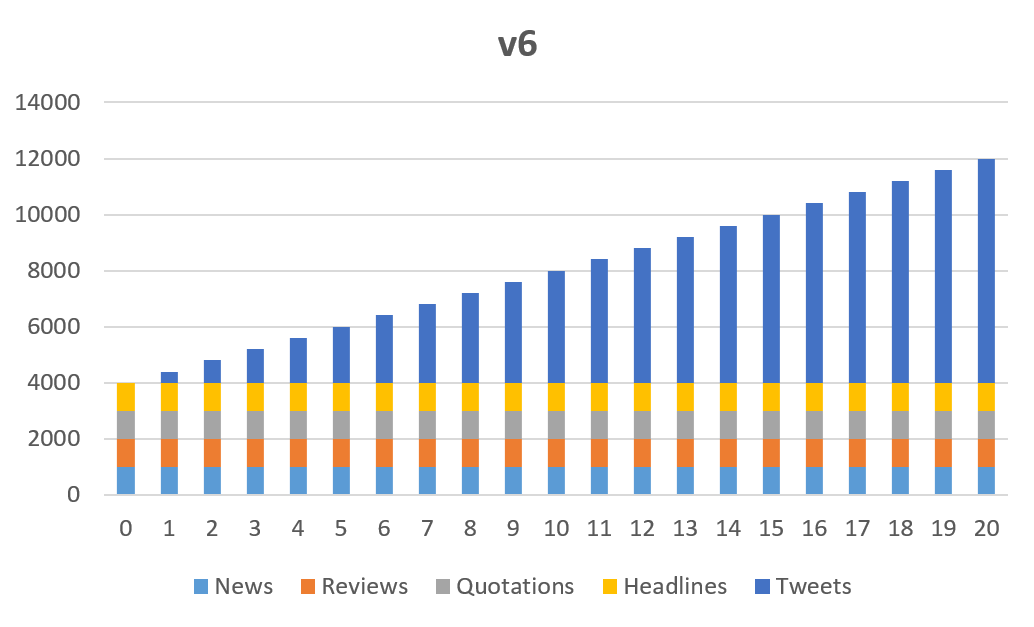
\includegraphics[width=0.7\textwidth]{img/Method_V6}
	\caption{Aufbau Experiment V6 - Tweets}
	\label{fig:Method_V6}
\end{figure}
Bei \ref{fig:Method_V6} ist die Zieldomäne SemEval Tweets, die Vorgehensweise für die Zieldomäne MPQ Reviews unterscheidet sich nicht.
\subsection{Experiment V7}
Im Experiment V7 wurde untersucht, wie stark sich die Performanz eines bereits trainierten CNN verbessert, wenn mit der Zieldomäne ähnlichen Daten weiter trainiert wird. Konkret bedeuted dies, es wird ein CNN für die Zieldomäne MPQ Reviews trainiert. Anschliessend wird in 10 Teilschritten mit einer steigenden Anzahl anderer Review Domänen (siehe Kapitel Daten), weiter trainiert.
%TODO Kapitel Date referenzieren?
%TODO insert Picture

\subsection{Experiment V8}
Das Experiment V8 dient als Baseline und somit Referenzwert für die Experimente V6 und V7.
Bei diesem Experiment wird nur mit den Daten der Zieldomäne trainiert und validiert \ref{fig:Method_V8}. Es dient als Anhaltspunkt, ob die Idee CrossDomain eine effektive  Steigerung der Performanz erbringen kann.
\begin{figure}[htbp]
	\centering
	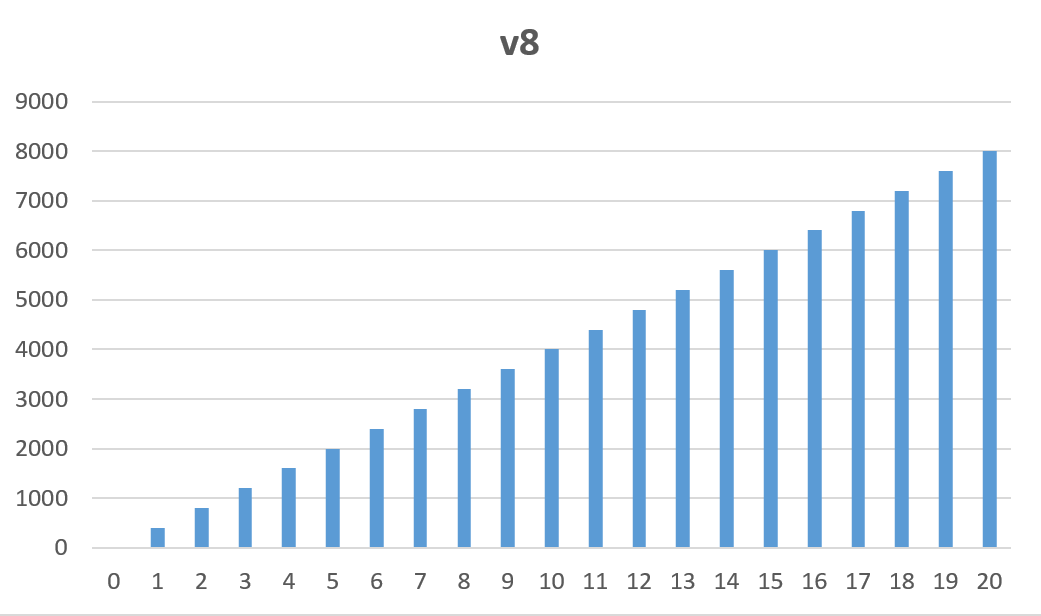
\includegraphics[width=0.7\textwidth]{img/Method_V8}
	\caption{Aufbau Experiment V8}
	\label{fig:Method_V8}
\end{figure}
%TODO CrossDomain in Glossar
$TODO F1_{pn} in Glossar 
